\documentclass{article}
\usepackage[margin=1in]{geometry}
\usepackage{comment}
\usepackage{tikz}
\usepackage{qtree}
\begin{document}
\tikzstyle{files}=[draw]
\tikzstyle{filelist}=[draw]
%%
\newcommand{\nl}{null}
\newcommand{\nls}{``''}
%%
\newcommand{\pro}{protected}
\newcommand{\pri}{private}
\newcommand{\pub}{public}
\newcommand{\ab}{abstract}
%%
\newcommand{\ob}{Object}
\newcommand{\st}{String}
\newcommand{\db}{double}
\renewcommand{\int}{integer}
\newcommand{\bo}{boolean}
\newcommand{\vo}{void}
%%
\newcommand{\St}{Struct}
%%
\newcommand{\oitem}[4]{#1 & #2 & #3 & #4 \\}
\newcommand{\citem}[3]{#1 & #2 & \plist{#3} & \\}%% constructors
\newcommand{\pitem}[2]{#1 & #2 \\}%% parameters
\newcommand{\mitem}[4]{#1 & #2 & #3 & \plist{#4}\\} %% methods
\newcommand{\amitem}[4]{\mitem{#1}{#2}{#3}{#4}}
%%
\newcommand{\classlist}[1]{\begin{tabular}{|l l l l|} \hline #1 \hline \end{tabular}}
\newcommand{\olist}[1]{ #1 }
\newcommand{\clist}[1]{ #1 }
\newcommand{\plist}[1]{\begin{tabular}{@{}l l} #1 \end{tabular}}
\newcommand{\mlist}[1]{ #1 }
\newcommand{\amlist}[1]{\mlist{#1}}
%%
\begin{center}
\begin{tikzpicture}[node distance = 2cm, auto]
	\node[files]	(Struct)				{Struct};
	\node[files]	(Data)		[right of=Struct]	{Data};
	\node[files]	(Calc)		[above of=Data]		{Calc};
	\node[files]	(Menu)		[right of=Data]		{Menu};
	\node[files]	(GUI)		[below of=Menu]		{GUI};

	\draw [->]	(Struct.east) -- (Data.west);
	\draw [->]	(Struct.north) -- (Calc.west);
	\draw [->]	(Data.north) -- (Calc.south);
	\draw [->]	(Data.east) -- (Menu.west);
	\draw [->]	(Calc.east) -- (Menu.north);
	\draw [->]	(Menu.south) -- (GUI.north);
\end{tikzpicture}
\end{center}

\Tree [ 
	.Struct [ 
		[ Steps Resting\_BPM [
			help
		].SInt
		[ Height Weight BF Activity\_Level ].SDouble 
		[ a b ].SString 
		[ a b ].Calc\_Abstract
	].
]
\begin{comment}
\begin{center}
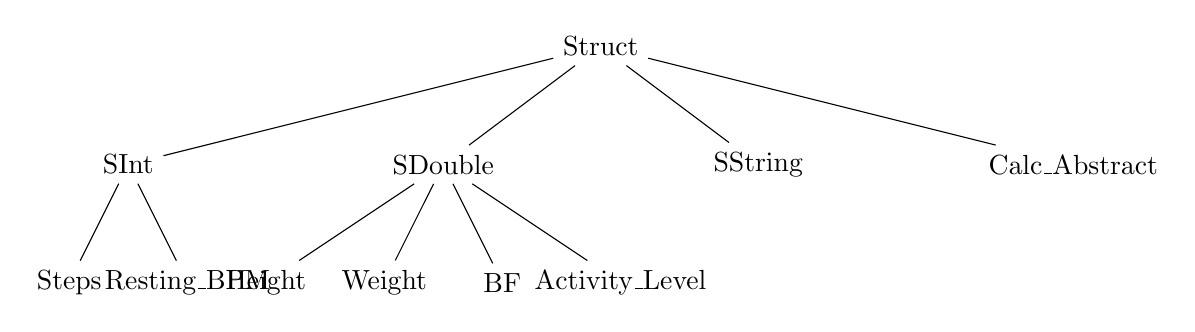
\begin{tikzpicture}
	\tikzstyle{level 1}=[sibling distance=4cm]
	\tikzstyle{level 2}=[sibling distance=1.5cm]
	\node	{Struct}
		child	{node	{SInt}
			child	{node	{Steps}}
			child	{node	{Resting\_BPM}}
			}
		child	{node	{SDouble}
			child	{node	{Height}}
			child	{node	{Weight}}
			child	{node	{BF}}
			child	{node	{Activity\_Level}}
			}
		child	{node	{SString}}
		child	{node	{Calc\_Abstract}};
\end{tikzpicture}
\end{center}
\end{comment}
\begin{comment}
%%\begin{tikzpicture}
%%	\node[filelist]	(Struct) {
	\classlist{
		\olist{
			\oitem{\pri}{\ob}{Struct\_Entry}{\nl}
			\oitem{\pri}{\st}{Struct\_Type}{\nls}
			\oitem{\pri}{\st}{Struct\_Units}{\nls}
			\oitem{\pri}{\bo}{Struc\_Lock}{false}
		}
		\\
		\clist{
			\citem{\pub}{\St}{\pitem{\st}{Type} \pitem{\st}{Units}}
			\citem{\pub}{\St}{\pitem{\ob}{o} \pitem{\st}{Type} \pitem{\st}{Units}}
		}
		\\
		\mlist{
			\mitem{\pub}{\ob}{GetEntry}{}
			\mitem{\pub}{\st}{GetType}{}
			\mitem{\pub}{\st}{GetUnits}{}
			\mitem{\pri}{\bo}{GetLock}{}
			\hline
			\amitem{\ab}{\bo}{SE}{\pitem{\ob}{o}}
			\mitem{\pro}{\vo}{SetEntry}{\pitem{\ob}{o}}
			\mitem{\pri}{\vo}{SetType}{\pitem{\st}{Type}}
		}
	}
%%	};
%%\end{tikzpicture}
\end{comment}
\end{document}
